\documentclass{article}
\usepackage{amsmath}
\usepackage{amssymb}
\usepackage{amsthm}
\usepackage{pgfplots}
\pgfplotsset{compat=1.18}
\usepackage{graphicx} % Required for inserting images
\usepackage[margin=1in]{geometry} % Adjusted margins for better readability
\usepackage{mathrsfs}
\usepackage[autostyle, english = american]{csquotes}
\MakeOuterQuote{"}

\usepackage{enumitem} % Improved formatting for lists
%\usepackage{xcolor} % Required for defining colors
\usepackage{mdframed} % Required for framing the NOTE sections
\usepackage[dvipsnames,svgnames,table]{xcolor}
\usepackage{hyperref}
\hypersetup{
     colorlinks   = true,
     citecolor    = gray
}

\usepackage{tocloft}

\renewcommand{\cftsubsecfont}{\normalfont\hypersetup{linkcolor=purple}}
\renewcommand{\cftsubsecafterpnum}{\hypersetup{linkcolor=blue}}
\newtheorem{definition}{Definition}
\newtheorem{note}{Note}

% Define a color for the box
\definecolor{lightblue}{RGB}{173, 216, 230}

% Define a framed box for notes
\mdfdefinestyle{MyFrame}{%
    backgroundcolor=lightblue,
    roundcorner=5pt,
    frametitlerule=true,
    frametitlebackgroundcolor=white,
    frametitlerulecolor=lightblue,
    innertopmargin=\topskip,
}

\definecolor{lightorangered}{RGB}{255, 200, 173}

% Define a framed box for notes
\mdfdefinestyle{HW}{%
    backgroundcolor=lightorangered,
    roundcorner=5pt,
    frametitlerule=true,
    frametitlebackgroundcolor=white,
    frametitlerulecolor=lightblue,
    innertopmargin=\topskip,
}

% Define a color for the box
\definecolor{lightblue}{RGB}{173, 216, 230}

% Define a framed box for notes
\mdfdefinestyle{MyFrame}{%
    backgroundcolor=lightblue,
    roundcorner=5pt,
    frametitlerule=true,
    frametitlebackgroundcolor=white,
    frametitlerulecolor=lightblue,
    innertopmargin=\topskip,
}
% Define a framed box for notes
\mdfdefinestyle{MyFrame}{%
    backgroundcolor=lightblue,
    roundcorner=5pt,
    frametitlerule=true,
    frametitlebackgroundcolor=white,
    frametitlerulecolor=lightblue,
    innertopmargin=\topskip,
}
%permuatation and comb
\newcommand*{\permcomb}[4][0mu]{{{}^{#3}\mkern#1#2_{#4}}}
\newcommand*{\perm}[1][-3mu]{\permcomb[#1]{P}}
\newcommand*{\comb}[1][-1mu]{\permcomb[#1]{C}}
% Define a box for class session dates
\usepackage[most]{tcolorbox}

\NewTColorBox{classsessionbox}{O{}}{
    colback=white,
    colframe=lightblue,
    arc=0pt,
    outer arc=0pt,
    leftrule=0pt,
    rightrule=0pt,
    toprule=0pt,
    bottomrule=0pt,
    boxrule=0pt,
    right=0pt,
    top=5pt,
    bottom=5pt,
    width=3cm, % Set the width as needed
    title={\textbf{#1}},
    fontupper=\small, % Adjust the font size as needed
    halign=flush right, % Align to the right
}

\usetikzlibrary{decorations.markings, arrows, arrows.meta}

\tikzset{
    midar/.style 2 args={
        very thick,
        decoration={name=markings,
        mark=at position .55 with {\arrow{latex}},
        mark=at position 0 with {\fill circle (2pt);},
        mark=at position 1 with {\fill circle (2pt);}}
        ,postaction=decorate,
    },
}
\makeindex

% Define a theorem style
\theoremstyle{definition}
\newtheorem{theorem}{Theorem}
\newtheorem{example}{Example}
\newtheorem{property}{Property}

\usepackage{listings}
\usepackage{color}
%\lstset{language=Python}
\definecolor{mygreen}{rgb}{0,0.6,0}
\definecolor{mygray}{rgb}{0.5,0.5,0.5}
\definecolor{mymauve}{rgb}{0.58,0,0.82}
\lstset{ %
  backgroundcolor=\color{white},   % choose the background color; you must add \usepackage{color} or \usepackage{xcolor}; should come as last argument
  basicstyle=\footnotesize,        % the size of the fonts that are used for the code
  breakatwhitespace=false,         % sets if automatic breaks should only happen at whitespace
  breaklines=true,                 % sets automatic line breaking
  captionpos=b,                    % sets the caption-position to bottom
  commentstyle=\color{mygreen},    % comment style
  deletekeywords={...},            % if you want to delete keywords from the given language
  escapeinside={\%*}{*)},          % if you want to add LaTeX within your code
  extendedchars=true,              % lets you use non-ASCII characters; for 8-bits encodings only, does not work with UTF-8
  frame=single,                    % adds a frame around the code
  keepspaces=true,                 % keeps spaces in text, useful for keeping indentation of code (possibly needs columns=flexible)
  keywordstyle=\color{blue},       % keyword style
  language=Python,                 % the language of the code
  morekeywords={*,...},           % if you want to add more keywords to the set
  numbers=left,                    % where to put the line-numbers; possible values are (none, left, right)
  numbersep=5pt,                   % how far the line-numbers are from the code
  numberstyle=\tiny\color{mygray}, % the style that is used for the line-numbers
  rulecolor=\color{black},         % if not set, the frame-color may be changed on line-breaks within not-black text (e.g. comments (green here))
  showspaces=false,                % show spaces everywhere adding particular underscores; it overrides 'showstringspaces'
  showstringspaces=false,          % underline spaces within strings only
  showtabs=false,                  % show tabs within strings adding particular underscores
  stepnumber=2,                    % the step between two line-numbers. If it's 1, each line will be numbered
  stringstyle=\color{mymauve},     % string literal style
  tabsize=2,                       % sets default tabsize to 2 spaces
  title=\lstname                   % show the filename of files included with \lstinputlisting; also try caption instead of title
}
\usepackage{floatrow}
\usepackage{tikz}
\usetikzlibrary{shapes.geometric, arrows,positioning}

\tikzstyle{startstop} = [trapezium, text width=5cm, minimum   height=1cm,trapezium left angle = 120,trapezium right angle=60,text centered, draw=black, fill=red!30]
\tikzstyle{io} = [trapezium, trapezium left angle=70, trapezium right 
angle=110, text width=3cm, minimum height=1cm, text centered, draw=black, fill=blue!30]
\tikzstyle{process} = [rectangle, text width=7cm, minimum height=1cm,    text centered, draw=black, fill=orange!30]
\tikzstyle{decision} = [diamond, text width=3cm, minimum height=1cm, text centered, draw=black, fill=green!30]
\tikzstyle{arrow} = [thick,->,>=stealth]


\title{Thermo Notes with Deeper Intuition... Hopefully}
\author{Shuvam Banerji Seal} % Adjusted to include the current date



\begin{document}

\maketitle
This is a series of notes, I am going to be making for my understanding and if anyone finds anything wrong with any of these notes then they are always free to contact me or contribute to this project of making the thermodynamics more understandable for all. A huge chunk of these notes have been inspired from the popular 20 lectures on thermodynamics by Buchdahl. The main goal of these notes are to find a deeper understanding of the thermodynamics frrom a more fundamental level interms of more rigorous mathematical construction. 

\tableofcontents

\section{Thermodynamic Systems}

\subsection{Definition and Contrast with Mechanical Systems}
What are we to understand here by a "thermodynamic system"? To answer this question at last we wisely remind ourselves first of what we mean by a "mechanical system", bearing in mind that we are not interested in the dynamical description of any changes which it may undergo. As a preliminary step, let us specifically contemplate a set of particles mutually joined by straight elastic rods. The whole arrangement is at first on a table before us, those particles which are in contact with the table being supposed immovable. To describe it in detail we need to give the values of a (finite) set of mutually independent variables, \( x_1, x_2, \ldots, x_n \), for example the coordinates of some of the particles referred to Cartesian axes, together with the lengths of some of the rods. Any such set of values is a configuration of the system. To say that the system has undergone some change from one (equilibrium) or another to another is merely to say that it has changed from one configuration, \( x_1, \ldots, x_n \), to another configuration \( x_1', \ldots, x_n' \). Any such change, then, consists in the displacement of parts of the system relative to each other, that is to say, it is a deformation of the system. Indeed, the fact that every change of any one of the variables \( x_1', \ldots, x_n' \) describes a certain deformation of the system is sufficiently important to attach a special name to variables which have this character: we call them \textbf{coordinates}. Now, two identically constructed systems of the kind just described above contain nothing happen to be the same as to all forms and purposes indistinguishable. It is precisely this property which characterizes the class of mechanical systems. In short, a system is \textit{mechanical}, and it relevant information about its equilibria is contained merely in the values of a set of \textit{\textbf{d-coordinates}}.

\subsection{Sample Thermodynamic System}
By way of contrast, we go on to consider a very simple example of a (phenomenological) system—let us always refer to it as our \textit{sample system}—which will turn out to be non-mechanical. It consists merely of a gas. Of course this has to be enclosed by a container; and since we want the volume of this to be variable we may simply take it to a cylinder permanently closed at one end and by a movable piston at the other. Further, there shall be some kind of stirrer inside the cylinder by means of which the gas can be agitated from without. Nevertheless, the gas alone constitutes the system; that is to say, neither the enclosure nor the stirrer are to be regarded as part of it.

\subsection{D-Coordinates and H-Coordinates}
Now, this system too can be \enquote{deformed}, namely by moving the piston.
\note{Superficially this deformation seems to be different from the kind of deformation encountered earlier, since we might argue that we are deforming the container, and that it is not part of the system. We can save the situation by noting that at the same time different parts of the gas are displaced relatively to each other.}
\\
\normalfont

A d-coordinate is therefore naturally associated with it, the value of which specifies the position of the piston. We denote it indiscriminately by \(x_i\) in particular it might, of course, be chosen to be the volume \(V\) occupied by the gas. No other non-redundant d-coordinate can be defined. Nevertheless even the most elementary observation shows that the equilibria of this system are not adequately described by the values of \(x_i\) alone. Indeed, we soon find that upon touching the system we may burn our fingers on one occasion and not do so on another. Clearly at least one other variable which is not a d-coordinate must be introduced. I shall call any such variable an \textbf{\textit{h-coordinate}}. In the case of our sample system only one of them is required, and it might, for instance, be taken to be the pressure \(P\) of the gas, but this choice is not mandatory.

\subsubsection{Key Distinctions: d vs. h Coordinates}
\begin{tabular}{|l|l|l|}
\hline
 & \textbf{d-Coordinates} & \textbf{h-Coordinates} \\ 
\hline
\textbf{Nature} & Mechanical deformation variables & Non-mechanical equilibrium variables \\ 
\hline
\textbf{Examples} & Volume \( V \), position \( x \), strain & Pressure \( P \), temperature \( T \), magnetization \\ 
\hline
\textbf{Role} & Describe spatial configuration & Encode internal state \\ 
\hline
\textbf{Work Relation} & Work \( \delta W = P_k \delta x_k \) & No direct work association \\ 
\hline
\end{tabular}
\subsection{Formal Definition of Thermodynamic Systems}
The state of affairs just described leads us quite generally to the understanding that a thermodynamic system is a system whose equilibria are specified by the values of a finite number of coordinates (i.e. variables) at least one of which is an h-coordinate. Although this definition appears to be very general, it does imply restrictions on the kind of physical systems which we admit for consideration. In particular, no substances can be present whose properties at a given time depend upon their previous histories. There is an infinity of such histories, whereas we are restricted to a finite number of coordinates.

\begin{itemize}
    \item \textbf{Mechanical System}: 
    \begin{itemize}
        \item Described entirely by \textit{d-coordinates} (deformation coordinates), e.g., positions of particles or lengths of elastic rods.
        \item Equilibrium states depend \textit{only} on these coordinates. 
        \item Example: A system of particles connected by rods; configurations are fully defined by Cartesian coordinates \( x_1, x_2, \ldots, x_n \).
    \end{itemize}
    
    \item \textbf{Thermodynamic System}:
    \begin{itemize}
        \item Requires \textit{at least one} \textbf{h-coordinate} (hidden coordinate) in addition to d-coordinates.
        \item h-coordinates capture non-mechanical properties (e.g., pressure, temperature) essential for equilibrium description.
        \item Example: A gas in a piston-cylinder system. Here, volume \( V \) (d-coordinate) is insufficient; pressure \( P \) (h-coordinate) is needed.
    \end{itemize}
\end{itemize}

\subsection{Thermal Equilibrium And Temperature:}
Consider a system defined by $f(P,V,M, Composition)$ (suppose a chamber of gas)\\
Generate an illustration of a chamber separated  by a rigid wall, and there are two pistons  on both sides.
The rigid wall is adiabetic.\\
The gas 1 and gas 2 can co-exist for any ($P_1, V_1$) and $(P_2, V_2)$.\\
If I do something on ($P_1, V_1$) then $(P_2, V_2)$ will also be affected.
Once they are connected by the diathermic wall, ($P_1, V_1$) and $(P_2, V_2)$ are not independent variables anymore.\\

But there, will be some relation $F(P_1, V_1,P_2, V_2) = 0$ \dots will hold only for the thermal equilibrium state.\\
Thermal equilibrium is the state achieved by two or more systems characterized by restricted set of parameters on having been separated by a diathermic wall.

\textbf{What is characterizing this Thermal equilibrium State?}
Defined such that the thermal equilibrium state is going to be only defined by one quantity ie temperature.


\subsection{Standard Systems and Their Constraints}
To keep everything as simple as possible, our main purpose being to gain insight into the subject, we shall very often impose a number of further restrictions, some or all of which are often implicitly taken for granted. The most important of these is that of the n coordinates exactly one is an h-coordinate. We further require that the effects of surface tension can be neglected and that likewise the effect of mutual long-range interactions between parts of the system can be neglected. The first of these assumptions is always satisfied if only the system is large enough; the second would not be justified in the context of a system so massive that the mutual gravitational attraction between its parts is comparable with other discrete operating within the system. Finally we require that when any one of the d-coordinates, \(x_k\), say, changes slowly enough by an amount $(\delta x_k)$, sufficiently small in absolute value, then the work $\delta W$ done by the system on its surroundings shall be proportional to $(\delta x_k)$, and the ratio \(P_k\), of $\delta W$ to $(\delta x_k)$, shall be a function of the coordinates alone. The functions \(P_1, \ldots, P_{n-1}\) are called the \textit{generalized forces} of the system.

A system which satisfies the various conditions just laid down will be called a \textit{standard system}. The large majority of systems considered in more or less elementary treatments of thermodynamics are of this kind. As which is sometimes not sufficiently emphasized. Our sample system is certainly a standard system with two coordinates. At times it is helpful to have a much less than 3 standard systems with n coordinates. Somewhat naively perhaps, we might take this to consist of \(n - 1\) sample systems, any one of the cylinders (taken to be metallic) being in contact with at least one of the others. Each sample system contributes one d-coordinate, so that there are \(n - 1\) of these and all. In addition we therefore need just one h-coordinate and this we may, for instance, choose to be the pressure \(P\) in any one of the cylinders. Occasionally the theory of a particular non-standard system can be reduced to that of standard systems. The possibility of being able to do so hinges on which particular defining condition of standard systems is not satisfied. It is, for example, not difficult to allow for the presence of surface tension when this is not negligible.

\subsubsection{Standard Thermodynamic Systems}
A system is \textbf{standard} if:
\begin{enumerate}
    \item It has \( n \) coordinates: \( n-1 \) d-coordinates and \textit{exactly one} h-coordinate.
    \item Surface tension and long-range interactions (e.g., gravity) are negligible.
    \item Work done during infinitesimal deformation is linear: 
    \[
    \delta W = \sum_{k=1}^{n-1} P_k \delta x_k
    \]
    where \( P_k \) are generalized forces (e.g., pressure, stress).
\end{enumerate}

\subsubsection{Example: Gas in a Piston-Cylinder}
\begin{itemize}
    \item \textbf{d-coordinate}: Volume \( V \).
    \item \textbf{h-coordinate}: Pressure \( P \).
    \item Work done: \( \delta W = -P \delta V \) (convention: work done \textit{by} the system).
\end{itemize}

\subsection{Coordinates and State Space}
\begin{itemize}
    \item A \textbf{state} \( \sigma \) is defined by a unique set of coordinates \( (x_1, \ldots, x_{n-1}; h) \).
    \item Equilibrium requires all coordinates to be well-defined. Non-equilibrium processes lack defined h-coordinates.
    \item Coordinates must be \textit{independent} and \textit{finite}, excluding history-dependent variables (e.g., hysteresis).
\end{itemize}

\subsubsection{Generalized Forces and Work}
For a quasi-static process:
\[
\delta W = \sum_{k=1}^{n-1} P_k \delta x_k
\]
\begin{itemize}
    \item \( P_k \): Generalized force conjugate to \( x_k \).
    \item Example: For \( x_k = V \), \( P_k = -P \) (pressure).
    \item Forces are state functions: \( P_k = P_k(x_1, \ldots, x_{n-1}; h) \).
\end{itemize}

\subsubsection{Non-Standard Systems}
Systems failing the standard criteria include:
\begin{itemize}
    \item \textbf{Multi-component systems}: Require additional coordinates (e.g., chemical composition).
    \item \textbf{Systems with long-range forces}: Gravitational or electromagnetic interactions dominate.
    \item \textbf{Small-scale systems}: Surface tension effects become significant.
\end{itemize}

\subsection{Notes on System Composition}
It remains to point out a small sin of emission. When referring to "a gas" I have throughout said nothing about the nature of this; it might well be a mixture of several gases, capable of reacting chemically with each other. In such a situation the chemical would come to be vitally interested in the proportions in which the various gases are present under conditions of equilibrium. However, the additional variables which must be introduced to describe the internal, i.e. physico-ehemical, constitution of a given system do not enter directly into the description of the interaction of the system with its surroundings. It is therefore preferable to deal with the required generalization of the theory after its general foundations have been laid.

\subsection*{Non-Standard Systems}
Systems failing the standard criteria include:
\begin{itemize}
    \item \textbf{Multi-component systems}: Require additional coordinates (e.g., chemical composition).
    \item \textbf{Systems with long-range forces}: Gravitational or electromagnetic interactions dominate.
    \item \textbf{Small-scale systems}: Surface tension effects become significant.
\end{itemize}

\subsection*{Critical Notes}
\begin{itemize}
    \item \textbf{Why h-coordinates?}: Mechanical coordinates alone cannot distinguish states with identical configurations but different internal energies (e.g., gas at same volume but different pressures).
    \item \textbf{Irreversibility}: Standard systems assume no memory (path-independence), but real systems may exhibit hysteresis (addressed later).
    \item \textbf{Generalization}: Chemical reactions or phase transitions require extending coordinates, but foundations first require mastering standard systems.
\end{itemize}

\subsection{Problems}
\begin{enumerate}
\item If the system is just a gas, can you think of an h-coordinate other than \( P \)?
\item A system consists of a block of iron on which work can be done not merely by compressing it but also by the action of an external magnetic field. Is the block a standard system?
\item Which, if any, of the following are standard systems: (i) the moon, (ii) a solution of rock salt in water, (iii) a gas consisting of oxygen and hydrogen, (iv) a rain drop? Discuss (iii) in detail.
\end{enumerate}


\section{States and Transitions, Adiabatic Isolation, Irreversibility}

\subsection{Definition of States}
We are already familiar with the meaning of the two kinds of coordinates of a thermodynamic system \( K \). In future we shall call any particular set of values of these a state \(\mathcal{G}\) of \( K \); for which reason the coordinates themselves are often also called ‘variables of state’. Of course, unless equilibrium obtains, h-coordinates are not defined, in the sense that experiment does not yield unique values which might be assigned to them. (For example, there is no single well-defined pressure which might be assigned to a gas in turbulent motion.) Accordingly it is meaningless to speak of a ‘non-equilibrium state’: a system not in equilibrium is simply in no state at all.

\note{Such a statement may look rather bewildering at first sight, considering that elsewhere one does apparently non-negligibly discuss ‘non-equilibrium states’. There is no contradiction. In one case we are operating strictly within the framework of the definitions of one theory; in the other, one is concerned with the definitions of another theory, e.g., fluid dynamics, and then what is meant by a ‘state’ is something altogether different.}\\
\normalfont

Concomitantly, since all quantitative statements of classical thermodynamics are about states, any predictions about the outcome of experiments involving non-equilibrium processes can be at best qualitative.

\subsection{Types of Transitions}
A change of any system \( K \) from one state to another will be called a transition of \( K \). In the course of a transition \( K \) may or may not be in equilibrium. When it is, i.e., when \( K \) goes through a continuous sequence of states, the transition is called pseudo-static; a terminology which reflects the fact that it must proceed ‘at an infinitesimal rate’,

\note{The phrase ‘at an infinitesimal rate’ of course cannot be taken literally, since otherwise we would be confronted with the unsavoury conclusion that a quasi-static transition occupies an infinite time interval. As in Note 1, we face the need to adopt a sensible interpretation. Here a transition proceeds ‘at an infinitesimal rate’ if it proceeds so slowly that the deviations from equilibrium are such that the system nevertheless behaves as if it were in equilibrium, i.e., to within experimental error the disequilibrium has no observable consequences.}\\
\normalfont
since otherwise the appearance of elastic waves, turbulence, and the like would not counter to the equilibrium which is supposed to obtain. If, further, in the course of a pseudo-static transition work is done by the forces \( P_k \) alone it is called quasi-static. (For example, transitions of a sample system brought about solely by turning the stirrer or alternatively solely by moving the piston, either process occurring at an infinitesimal rate, or as pseudo-static and quasi-static, respectively.) Finally, a transition such that \( K \) is not in equilibrium in the course of at least a part of it is called non-static.

Special conditions are frequently imposed upon transitions which restrict their generality. For example, when all d-coordinates of \( A \) are kept fixed by prescription the transition is isometric; if we merely require their final values to be the same as their initial values we call it weakly isometric. Further, a transition is infinitesimal if the final state, and in the case of a quasi-static transition every intermediate state, is sufficiently close to, i.e., lies in the neighbourhood of the initial state.

\note{Physicists often rely on intuition for an understanding of this definition. That is, indeed, often quite good enough. What is in fact usually meant when speaking of the neighbourhood? An \(\epsilon\)-neighbourhood of \(\Theta\), with \(\epsilon\) being some preassigned positive number. Having chosen a set of coordinates of \( K \) and the units in which these are to be measured, it will suffice to take an \(\epsilon\)-neighbourhood of \(\Theta[x_1, \ldots, x_n]\) to consist of all states \(\Theta[x_1', \ldots, x_n']\) such that \(|x_1' - x_1| + |x_2' - x_2| + \cdots + |x_n' - x_n| < \epsilon\). In the context of infinitesimal transitions, by "transitions between neighbouring states", \(\epsilon\) must be taken to be sufficiently small. Thus, if something is said to be true in every neighbourhood of \(\Theta\), it means that it is true no matter how one chooses \(\epsilon\); in particular, that it will be true for arbitrarily small values of \(\epsilon\).
}\\

\normalfont
Again, a most prominent position is occupied in the theory of the class of so-called adiabatic transitions. To define these we must first clearly understand what is meant by adiabatic isolation.

\subsection{Adiabatic Isolation}
To this end, let us first think about the homely example of an aluminium container filled with water and ice cubes. Upon placing it in a refrigerator we may find that after some time the water has also turned into ice. On the other hand, they've placed the container over the flame of a gas burner the ice cubes would have melted, the evaporation of some or all of the water quite apart. Now contrast this behaviour with what we observe when the aluminium container is replaced by a high-quality thermos flask. True, the ultimate behaviour of the water ice mixture is the same, yet an altogether different time scale is involved. For instance, upon placing the flask in the refrigerator we may have to wait for days for the water to freeze. It is therefore not unreasonable to suppose that better and better ‘thermos flasks’ could be constructed until we end up with one which is such that it is to all intents and purposes altogether impossible to melt the ice or freeze the water contained within it merely by placing it into appropriate surroundings.
\note{We are again confronted with an idealization, and we cannot be sure that it is warranted. After all, it is certainly true that in practice we cannot construct an ‘ideal’ thermo flask. We may still think it ‘reasonable’ to allow its introduction into the theory, especially as only a question of time scale appears to be involved—and we already encountered difficulties surrounding this several times before. Still, one has to be careful: what is ‘reasonable’ today may not be ‘reasonable’ tomorrow. Sudden changes in attitude have occurred in the history of physics, for example following upon the introduction of the Heisenberg Uncertainty Principle, the Restricted Relativity Principle, and the like.}\\
The only way to melt the ice is to some mechanical process, not by shaking or stirring.
\normalfont
The particular example just discussed leads us to the following general definition: an enclosure is called adiabatic (a) the equilibrium of a system contained within it can only be disturbed or mechanical means. An enclosure which is not adiabatic is called diathermic. Any doubt as to what constitutes ‘mechanical means’ is removed by prescription; examples are shaking, stirring, the movement of a piston (or more generally any deformation of the system), and the passage of an electric current.

\subsection{Adiabatic Transitions and Work}
A system which is contained within an adiabatic enclosure is adiabatically isolated, and we represent it by the symbol \( K_0 \). The transitions of \( K_0 \) are adiabatic transitions, whether quasi-static or not. Here we should be clearly aware of the distinction between isolation on the one hand and adiabatic isolation on the other. The latter condition is the weaker of the two since it does not forbid arbitrary mechanical interaction between the system and its surroundings. In other words, a system can certainly make up work on its surroundings in the course of an adiabatic transition. (We note in passing that the 4-coordinates of an adiabatically isolated system can still be varied at will.)

There are evidently two kinds of possible interactions between a system and its surroundings. When it is adiabatically isolated, the interaction must be mechanical, and it necessarily involves large-scale, observable motions in the surroundings, such as the displacement of levers, pistons and the like [Note 7]. In the absence of adiabatic isolation the interaction may, however, be partly or wholly non-mechanical—synonymously: adiabatic or thermal—and no such observable, large-scale motions need occur.

\subsection{Reversibility and Irreversibility}
It remains to talk about another division of transitions into two broad classes, the distinction between which lies at the root of thermodynamics. To this end we must first ask ourselves what one might understand by the ‘reversal’ of a transition. We contemplate in the first instance only adiabatic transitions. Then the reversal of a transition of \( K_0 \) from a state \(\mathcal{G}\) to a state \(\mathcal{G}'\) simply means a subsequent transition which restores the system (adiabatically) to its initial state \(\mathcal{G}\). This may turn out to be in fact impossible; in that case the original transition is called irreversible, otherwise it is reversible. In the absence of adiabatic isolation, reversal can clearly no longer mean the mere restoration of \( K \) to its initial state since this can always be achieved by allowing it to interact suitably with its surroundings. Evidently an additional condition must be satisfied. It is this: that after the restoration of \( K \) to its initial state no overall changes in the surroundings remain as the result of the process as a whole. Of course it is not a priori obvious that there are any irreversible transitions of an arbitrarily selected system at all. That there are is, in effect, one of the central laws of nature which will require us a good deal later on, especially in the next lecture.

Although quasi-static transitions of a standard system \( K \) are reversible it is not at all obvious that all reversible transitions of \( K \) must be quasi-static. It is in fact an experimental result that they are so in the overwhelming majority of cases. There are, however, ‘abnormal systems’ which behave differently in this and other respects. We shall return to these at the end of the course.

\subsection{Problems}
\begin{itemize}
\item 3.1 Describe what manifest differences there are between the outcomes of the following alternative transitions of our sample system, i.e. of a gas contained in an adiabatically enclosed cylinder supplied with a piston in the usual way: (i) the piston is moved to and fro very slowly at constant speed so that the volume of the gas is first doubled and then reduced to its initial value; (ii) the volume is first doubled by sudden withdrawal of the piston and then restored to its initial value. (The surroundings of \( K_a \) may be thought of as some external mechanical device.)
\item 3.2 In the case of the system of Problem 2.2, leaving hysteresis aside as irrelevant here, do you consider the interaction via the magnetic field to be mechanical or thermal?
\item 3.3 A system consisting of a gas contained in an enclosure is being stirred by means of a clockwork mechanism powered by a spring. What is the number of coordinates whose values constitute a state at any given time?
\item 3.4 Can a purely mechanical system undergo ‘irreversible changes’?
\item 3.5 A system \( K \) consists of two gases each contained in an adiabatic enclosure, the two enclosures being in mutual contact. \( K \) is not a standard system. Why not?
\end{itemize}



\section{The Second Law, Entropy and The Entropy Principle}

We regard the irreversibility of a given transition of a system as being characteristic of the behaviour of the system as such, not of its surroundings. To this extent the character of its interactions with the surroundings is irrelevant. Both as a matter of principle and to aid our understanding and insight we therefore temporarily contemplate only the simplest kind, namely those which are mechanical. In short, we confine our attention to adiabatic transitions.

Let us consider again our sample system and suppose that the surroundings do work on this system \(K_0\) for a certain time by means of the stirrer. As a result the pressure of the gas will have increased—this is merely a matter of observation—whilst the volume has remained constant. To reverse the transition would require the reduction of the pressure to its initial value, the volume than also having its initial value. How is this to be done? It is useless to turn the stirrer since irrespectively of whether we turn it this way or that, fast or slowly, more work will be done on \(K_0\) and the pressure will increase further. We may, on the other hand, seek to reduce it by withdrawing the piston but then we end up with an increased volume. Upon restoring it to its original value by pushing the piston in we regain either the intermediate value of the pressure, if the to-and-fro process proceeded at an infinitesimal rate, or an even greater pressure if it did not [cf. Problem 3.1]. In short, the original state of \(K_0\) cannot be restored, i.e., the transition under discussion is irreversible.

We can shift the emphasis a little by rephrasing this conclusion as follows. Given some initial state \(\mathcal{G}\) there is a whole class of states of \(K_0\) such that no transition from \(\mathcal{G}\) to any one of these states is possible. On particular, if \(\mathcal{G}\) is the state \(V\), \(P\) then certainly all those states \(|V', P'\) such that \(V'=V,P'<P\) belong to the class of states in question, no matter how small \(|P-P'|\) may be). We can sum up the whole content of the conclusion reached so far somewhat formally as follows: in any neighbourhood of a given state \(\mathcal{G}\) of \(K_0\) there are states \(\mathcal{G}'\) inaccessible from \(\mathcal{G}\).

\note{The first of them is usually known as the Principle of Carathéodory. It is largely equivalent to the traditional statements of the Second Law of Thermodynamics. Its experimental confirmation is mostly indirect: no-one in his senses would suppose that, as a practical proposition, its validity could be tested directly. In any event, such a remark might be made about many laws of physics.
}\\
\normalfont
Moreover, it is obvious in the case of the sample system under discussion that if the state \(\mathcal{G}'\) is adiabatically inaccessible from \(\mathcal{G}\), then \(\mathcal{G}\) is (adiabatically) accessible from \(\mathcal{G}'\). Setting our special system aside now, the results of innumerable experiments confirm that the two main conclusions just stated hold quite generally for (standard) systems of arbitrary complexity [Note 8].

\subsection{Empirical Entropy Function}
Suppose now that \(\mathcal{G}\) and \(\mathcal{G}'\) are arbitrarily selected states of some adiabatically isolated system \(K_0\) such that \(\mathcal{G}\) is inaccessible from \(\mathcal{G}'\) (and therefore \(\mathcal{G}'\) accessible from \(\mathcal{G}\)). This specification evidently contains a time order in the following sense: given merely that \(K_0\) was in the state \(\mathcal{G}\) at some time and in the state \(\mathcal{G}'\) at some other time we can say that \(\mathcal{G}'\) was necessarily the later state. With this idea of an ordering amongst the states of \(K_0\) in mind, let us contemplate some ungoedness set of selected states \(\mathcal{G}_1\), \(\mathcal{G}_2\), \ldots of \(K_0\). We first represent \(\mathcal{G}_1\) by an arbitrarily situated point \(p_1\) on a straight line. Next \(\mathcal{G}_2\) is represented by a point \(p_2\) of which we merely require that it lie to the right of \(p_1\) if \(\mathcal{G}_1\) is inaccessible from \(\mathcal{G}_2\), to the left of \(p_1\) if \(\mathcal{G}_2\) is inaccessible from \(\mathcal{G}_1\), and that it be coincident with \(p_1\) if \(\mathcal{G}_1\) and \(\mathcal{G}_2\) are mutually accessible. (The three cases respectively correspond to the transition from \(\mathcal{G}_1\) to \(\mathcal{G}_2\) being irreversible, impossible, and reversible.) We continue this construction by representing the states \(\mathcal{G}_3\), \(\mathcal{G}_4\), \ldots by points \(p_3,p_4,\ldots\) in turn in such a way that, if \(p_j\) and \(p_k\) are any two points, \(p_k\) lies to the right of \(p_j\) to the left of \(p_j\), or coincides with \(p_j\) according as the transition from \(\mathcal{G}_j\) to \(\mathcal{G}_k\) is irreversible, impossible or reversible, respectively. Finally we attach to each such point a number which can be chosen at will subject to the sole condition that these numbers increase monotonically as we proceed from left to right. (Coincident points of course take the same number.)

Each state is a set of values of the coordinates \(x_1,\ldots,x_n\) of the system. The procedure just described therefore amounts to the definition of a certain state-function \(s(x_1,\ldots,x_n)\) (or simply \(s(\mathcal{G})\)), for this is only another way of saying that a correspondence has been established between the set of states \(\mathcal{G}_1\), \(\mathcal{G}_2\), \ldots and a set of numbers \(s_{1}, s_2\ldots\).

\note{Even now it should be emphasized that the function \( s \) is so far defined only on the discrete set of states \(\Theta\), \(\Theta_x, \ldots\). Questions of its continuity or differentiability are therefore as yet beside the point. The construction we have carried out could of course be undertaken also in the context of other systems for which ‘states’ have been defined, as, for example, in the case of a dynamical particle system, the state being taken as a set of values of position coordinates and of the corresponding velocities. However, the construction is then empty in the sense that all representative points will coincide, i.e., \( s \) is a fixed constant. To a large extent, the essential content of the Second Law (to be stated shortly) is that for thermodynamic states the construction is, in fact, not empty.
}\\
\normalfont
Any particular \(\mathcal{G}_j\) is labelled by a number \(s_j=s(\mathcal{G}_j)\), this labeling having the fundamental property that a transition from a state \(\mathcal{G}_j\) to a state \(\mathcal{G}_k\) is possible if and only if \(s_j\leq s_{k}\) (equally implying reversibility). We call \(s_j\) the \textit{empirical entropy} of \(\mathcal{G}_j\) (or of \(K\) in the state \(s(\mathcal{G}_j)\) and $s(\mathcal{G}_j)$ the \textit{empirical entropy function} of \(K\). Evidently if \(K_0\) undergoes a transition from \(\mathcal{G}_j\) to \(\mathcal{G}_k\), the empirical entropy of the final state can never be less than that of the initial state.

\subsection{Continuum of States and the Second Law}
Now, however large the set of states \(\mathcal{G}_1\), \(\mathcal{G}_2\), \ldots may be—it may even be infinite—it certainly does not contain all possible states in which \(K_0\) may find itself; they form a continuum.

\note{That the set of possible states of \( K_s \) is continuous whereas the set of quantum mechanical states of a bound system is discrete must on no account be thought to involve a contradiction: quantum states are not the states we are talking about, and a given ‘quantum state’ indeed depends continuously on the value of the \( d \)-coordinates which go to make up a thermodynamic state when they vary at an infinitesimal rate.
}\\
\normalfont
It is therefore impossible to construct a labeling of the states of \(K_0\) by the simple method adopted.

\note{Since the passage of an electric current through \( K \) was taken to constitute mechanical interactions, this statement would appear to be true when the source of the current is an electric generator but false when it is a battery. To be on the safe side, we should supplement ‘motions’ with the words ‘or chemical reactions’.}\\
\normalfont
For the distinction between the continuum of states and a sufficiently large set \(\mathcal{G}_1\), \(\mathcal{G}_2\), \ldots selected from another then, however important mathematically, is physically vacuous. Being loath to abandon the particular conceptual approach which led to easily to an understanding of the idea of entropy we cut the Gordans knot by simply declaring that such a good function \(s(x_1,\ldots,x_n)\) [Note 11] with the required properties always exists. In short, we lay down the following law, intended to be a formulation of the \textit{Second Law of Thermodynamics} (so called for historical reasons):

\begin{quote}
\textbf{\textit{There exists an ordering amongst the states of any thermodynamic system \(K\), reflected in the existence of a function \(s\) of the coordinates of \(K\) such that if \(s',s''\) are the values of \(s\) for arbitrarily selected states \(\mathcal{G}'\), \(\mathcal{G}''\) of \(K\), then \(\mathcal{G}''\) is adiabatically inaccessible from \(\mathcal{G}'\) if and only if \(s''<s'\).}}
\end{quote}

We call \(s\) an \textit{empirical entropy function} of \(K\), as before, and that it is a good function is left understood. It is not uniquely determined, in as far as \(\sigma(s)\) is an equally acceptable empirical entropy function if \(\sigma(s)\) is any good monotonically increasing function of \(s\). This arbitrariness runs precisely parallel with that which we encountered when we were numbering a set of discrete representative points on a line: the sole condition which these numbers had to satisfy was that they should increase monotonically from left to right. Nonetheless, there are preferred functions \(\sigma\), but it is perhaps better to deal with these later on. At any rate, from the outset the Second Law in its present form places explicit emphasis upon the existence of irreversible processes. In doing so, it directly attaches an intuitively transperent meaning to entropy without the encumbrances of having to take into account any of the other principal laws of thermodynamics and the various quantites such as energy or heat, whose definitions derive from them.

Finally, according to the Second Law the transition from $\mathcal{G}'$ to $\mathcal{G}''$ is possible only and only if $s''\leq s'$ i.e. \textit{the entropy of the state of an adiabatic transition is never less than that of the initial state}. This is nothing other than the \textbf{Principle of Increase of Entropy}, basically a rewording of the second law.

\subsection{Problems}
\begin{itemize}
\item 4.1 Experiment shows that \(PV^\gamma\) is constant during a reversible adiabatic transition of a certain gas (\(\gamma\) is given constant \(> 1\)). What states are adiabatically inaccessible from the state \(\mathcal{G}[P, V]\)?
\item 4.2 Is there any substantial reason why in the statement of the Second Law the inequality \(s'' < s'\) could not be replaced by \(s' > s''\)?
\item 4.3 Strictly speaking nor form of the Second Law contains an omission. Can you say what it is, bearing in mind what you know about mechanical systems?
\end{itemize}


\section{The First Law, Energy and Heat}

We return briefly to mechanical systems. Given any configuration, we know all about the forces which hold the system in equilibrium, such as gravity, elastic forces in connecting rods, and the like. In a change from one configuration to another, i.e. in the course of deforming the system, a certain amount of work will, in general, have to be done against these forces, and this depends solely on the initial and final configurations.

\note{This statement is in practice not rigorously true. It represents an idealization in which at least the assumption that all elastic substances in the system are ‘perfectly elastic’ is satisfied. As remarked earlier, for instance in \textit{Note 6}, one always has to be careful with idealizations; in the present context not least because one runs the risk of a circular argument which in the end says no more than that a certain statement is true when it is true. What it all amounts to here is this: in a strictly mechanical system, all elastic substances must be perfectly elastic, and a perfectly elastic substance is such that the amount of work done on it depends solely upon the deformation it has undergone. This therefore is a definition, and we can then determine by experiment whether a given substance is perfectly elastic or not. In practice, it must of course suffice that it should, under appropriate circumstances, have the property only within experimental error. Incidentally, the system must be both initially and finally at rest. Evidently, any change in configuration must occur ‘sufficiently slowly’ or else vibrations will be set up, and the only way to stop these is by means of frictional forces. Then the statement under discussion would again be false.
}\\
\normalfont
We can put this in another way: for any mechanical system there exists a function \(E\) of its coordinates such that the work done on the system in any change of configuration is equal to the increase in the value of \(E\). This function, called the energy of the system, is defined only to within an arbitrary additive constant. Evidently if a particular change of configuration is such that the work done happens to be zero, then the initial and final values of \(E\) are equal; this is what is meant here by the conservation of energy. In short, the energy of every mechanical system is conserved; but in saying this we must bear in mind that \(E\) is solely a function of \(\infty\) coordinates.

\note{A conservation law governing some physical quantity \( q \) declares that as the system with which it is associated pursues its history, the value of \( q \) remains constant; or sometimes, more weakly, that the value of \( q \) in the remote future will be equal to its value in the remote past. Thus, given the initial value of \( q \), one knows its value at all times (or at least in the remote future) without necessarily having to know anything about the details of the evolution of the system—details which may be unavailable in practice or sometimes even in principle.}\\
\normalfont
\subsection{Thermodynamic Systems and Work}
We now go over to thermodynamic systems. Work is done here, too, when the \(\infty\) coordinates vary. It is, however, not true that the amount of work in a transition depends solely on the deformation it has undergone, i.e. on the extent to which the \(\infty\) coordinates have varied. That this is so becomes obvious on reflecting that work can be done on the system simply by stirring it, and in that process the values of the \(\infty\) coordinates do not change at all. Furthermore there is reason why, in general, the final values of the \(\infty\) coordinates should differ from their initial values. As far as the system is concerned, the work done on it has apparently simply ‘disappeared’. At first sight it therefore looks as if no energy function could usefully be ascribed to a thermodynamic system. How is this unhappy situation to be rescued?

\subsection{First Law of Thermodynamics}
A possible answer to the preceding question suggests itself as soon as we recall that a thermodynamic system \(K\) can interact in two ways with its surroundings, namely mechanically and thermally (i.e. non-mechanically). Once again we are led to exclude thermal interactions; that is to say we consider only adiabatic transitions for the time being. In this situation the results of innumerable experiments show that the amount of work done by a system in an adiabatic transition depends on the terminal states alone.

This, indeed, is the so-called First Law of Thermodynamics. To leave our room for doubt, let it be emphasized that according to this law the work \(W\) done does not depend on the manner in which the transition of \(K_a\) between given states proceeds, i.e. whether it is reversible or not, and so, in particular does not depend upon any intermediate states through which \(K_a\) may happen to pass in the course of the transition.

\subsection{Energy Function and Heat}
Further progress is now quite straightforward. Not to be hindered by mere appearances, we first simplify the notation a little by writing, in appropriate circumstances, \(x\) for the whole set \(x_1, \ldots, x_m\) and of course \(y\) for \(y_1, \ldots, y_m\) and so on. A state \(\mathcal{G}^+\) is then a set of values \(x^*\) of the coordinates \(x\), and this is occasionally made quite explicit by writing \(\mathcal{G}\) [\(x\)] placed \(\mathcal{G}^+\) alone. Now, according to the First Law, the amount of work done by a system in any adiabatic transition from a state \(\mathcal{G}^+[x^*]\) to a state \(\mathcal{G}^-[x^*]\) is merely a function \(F(x^*, x^*)\) of these states (if depending of course on the structure of the given system). Hence if \(K_A\) undergoes a transition from \(\mathcal{G}[x]\) to \(\mathcal{G}^+[x^*]\) and then a subsequent transition from \(\mathcal{G}^+[x^*]\) to \(\mathcal{G}^-[x^*]\) the total amount of work done by it is \(F(x^*, x^*) + F(x^*, x^*)\). However, we know from the outset that in any transition from \(\mathcal{G}^+\) to \(\mathcal{G}^-\) the work done by \(K_B\) is \(F(x^*, x^*)\), so that the identity
\[F(x^*, x^*) + F(x^*, x^*) = F(x^*, x^*) \]
must be satisfied for all values \(x^*\) of the coordinates of the intermediate state. In other words, in forming the sum on the left the \(x^*\) must cancel out and the only possible if \(F(x^*, x^*)\) has the generic form
\[F(x^*, x^*) = U(x^*) - U(x^*) \]
where \(U\) is a certain function which is as usual assumed to be a good function. It is called the internal energy function of \(K\) or, more briefly, its energy. It is defined, i.e., can be measured, only to within an arbitrary additive constant. Thus, simply expressed, the First Law declares that an adiabatic transition the work \(W_0\) does by the system is equal to the decrease \(-\Delta U\) of its energy:
\[W_0 + \Delta U = 0 \]
We thus have a situation which is strongly reminiscent of that encountered in the case of mechanical systems.

Now let the condition of adiabatic inclusion be abandoned. When \(K\) undergoes some transition between given states \(\mathcal{G}^+\), \(\mathcal{G}^-\) the best we can do is to measure the amount of work \(W\) actually done by \(K_B\); there is no reason why it should be just \(W_0\). In other words, the quantity \(W + \Delta U\) will in general fail to vanish. It is therefore usual to introduce the abbreviation
\[Q = W + \Delta U \]
and for historical reasons one rather qualifies calls \(Q\) the 'heat absorbed by \(K'\) in the transition. However, let us be clear that this heat \(Q\) is simply the difference between two mechanical quantities, namely the difference between the amount of work done by the system in the actual transition between given states and the amount of work which would have been done in an adiabatic transition between the same states [Note 15]. In particular, a transition is adiabatic if and only if the least is translated between the system and its surroundings in the course of it. This is of course not a definition: it is merely a somewhat trivial consequence of the First Law, and to state the latter we already had to know what we meant by an adiabatic transition.

\subsection{Properties of Energy}
We have already supposed that \(U\) is a good function.

\note{By a ‘good’ function I mean a function which is single-valued, continuous, and sufficiently often differentiable, at least within some finite neighbourhood of a given state of interest. Here again it is best to postulate that \( s \) is a good function. Given only the existence of states inaccessible from a given state and the non-existence of pairs of mutually inaccessible states, together with assumptions about neighbourhoods of states, one can, by sophisticated arguments, prove the existence of a continuous function \( s \). However, one still cannot prove its differentiability, so that the whole endeavour is in the end just a wasteful exercise. In any event, functions which turn up in physics are often simply assumed to be good: whether they really are or not can obviously not be tested by direct experiment. Where discontinuities appear to occur, one simply has to analyse them by special arguments.}
\normalfont

Apart from this, experiment shows that the energy of any given system has a least value, i.e. it has a lower bound. On the other hand the energy of the vast majority of systems has no upper bound. Unless the contrary is stated explicitly, I shall therefore suppose throughout that the energy of any system can be increased indefinitely, and that this can indeed be done even by means of isometric processes alone.

\subsection{Perpetual Motion and Additivity}
A 'perpetual motion machine of the first kind' is intended to be some cyclic mechanism, however complex, which can continue indefinitely to do work on its surroundings with which it can interact only mechanically. However, at the end of any number of cycles, being again in its initial state, \(\Delta U = 0\) and, since \(Q\) also vanishes, \(W = 0\). There are therefore no such mechanisms; and the failure of all attempts to construct them is simply evidence of the validity of the First Law, or, as one sometimes says, of the conservation of energy [Note 15].

Finally, a word about the additivity of energy. Suppose we consider two systems \(K_A\) and \(K_B\) jointly and regard them as constituting a compound system \(K_C\). It does not matter whether \(K_A\) and \(K_B\) are in mutual contact or not. If they are standard systems the work done by \(K_C\) in any transition is simply the sum of the amounts of work done separately by \(K_A\) and \(K_B\); for on the one hand there are no surface forces which might have to be taken into account when they disappear to their contact, whilst on the other, their relative positions are irrelevant because of the absence of mutual long-range interactions. Since energy changes and subsequently heat are defined solely in terms of the amounts of work done on the various systems under the appropriate conditions, it follows at once that \(Q_C = Q_A + U_B\) and \(Q_C = Q_A + Q_B\). In short, in this sense energy and heat are additive, but we must not forget that we have only standard systems in mind.

\subsection{Problems}
\begin{itemize}
\item 5.1 On any reasonable time scale the earth will continue indefinitely to revolve about the sun in a nearly elliptic orbit. Is this an example of a perpetual motion machine?
\item 5.2 A rigid adiabatic enclosure is divided into two parts by means of an internal partition. Initially the first compartment contains a gas whilst the second is evacuated. The partition is subsequently removed so that the gas will fill the whole enclosure. What can you say about the value of \(\Delta U\)?
\item 5.3 For the sake of argument, suppose that a system consists of a fluid contained in a rigid adiabatic enclosure. (The system is artificial in that there are no deformation coordinates. On the other hand, the usual stirrer is to be present.) Determine an empirical entropy function.
\end{itemize}





\section{Class Notes:}
TD (Total Density) of the sample mixture = $\frac{V}{n_A + n_B}$\\

Suppose there are $i$ components in the gas such that for some $m>0 $ and $m$ being an integer $i \leq m$, then we can also define the partial molar volume as $V_i$ for the $i^{th}$ component. 

Now we can define $F$ as a first-order homogeneous function in $n_i$ as $F(T,P, n_1, \ldots, n_m)$, where $T\rightarrow Temp$, $P\rightarrow Pressure$, and $n_i$ is the total number of moles for the $i^{th}$ component.



\\\\\\\\\\\\\\\\\\\\\\\\\\\\\\\\\\\\\\\\\\\\\\\\\
\begin{mdframed}[style=MyFrame, frametitle={Definition of Homogeneous Functions}]
    

A function $F(x_1, x_2, \dots, x_n)$ is said to be \textbf{homogeneous of degree $k$} if for any scalar $\lambda$, it satisfies:

\begin{equation}
    F(\lambda x_1, \lambda x_2, \dots, \lambda x_n) = \lambda^k F(x_1, x_2, \dots, x_n)
\end{equation}

where $k$ is a constant called the \textbf{degree of homogeneity}. This means that when all arguments are scaled by $\lambda$, the function itself scales by $\lambda^k$.
\\
\\
\textbf{Examples of Homogeneous Functions}\\
1. Homogeneous of degree 1:
   \begin{equation}
       F(x, y) = x + y
   \end{equation}
   Scaling $x$ and $y$ by $\lambda$ gives:
   \begin{equation}
       F(\lambda x, \lambda y) = \lambda x + \lambda y = \lambda F(x, y)
   \end{equation}
   Thus, $F$ is homogeneous of degree 1.

2. Homogeneous of degree 2:
   \begin{equation}
       F(x, y) = x^2 + y^2
   \end{equation}
   Scaling $x$ and $y$ by $\lambda$:
   \begin{equation}
       F(\lambda x, \lambda y) = (\lambda x)^2 + (\lambda y)^2 = \lambda^2 (x^2 + y^2) = \lambda^2 F(x, y)
   \end{equation}
   So, $F$ is homogeneous of degree 2.
\\
\\
\textbf{First-Order Homogeneous Functions}\\
A function is \textbf{first-order homogeneous} if it is homogeneous of degree $1$, meaning:
\begin{equation}
    F(\lambda x_1, \lambda x_2, \dots, \lambda x_n) = \lambda F(x_1, x_2, \dots, x_n)
\end{equation}

In thermodynamics, extensive properties such as \textit{volume} ($V$), \textit{energy} ($U$), and \textit{Gibbs free energy} ($G$) are first-order homogeneous functions.

For instance, if $G$ represents Gibbs free energy:
\begin{equation}
    G(T, P, n_1, n_2, \dots, n_m)
\end{equation}
then, due to extensivity:
\begin{equation}
    G(T, P, \lambda n_1, \lambda n_2, \dots, \lambda n_m) = \lambda G(T, P, n_1, n_2, \dots, n_m)
\end{equation}
\\
\\
\textbf{Euler’s Theorem for Homogeneous Functions}
\\
Euler’s theorem states that if $F(x_1, x_2, \dots, x_n)$ is a homogeneous function of degree $k$, then:

\begin{equation}
    \sum_{i=1}^{n} x_i \frac{\partial F}{\partial x_i} = k F
\end{equation}
\\
\\

\textbf{Derivation of Euler’s Theorem}
\\
Since $F$ is homogeneous of degree $k$:
\begin{equation}
    F(\lambda x_1, \lambda x_2, \dots, \lambda x_n) = \lambda^k F(x_1, x_2, \dots, x_n)
\end{equation}

Differentiating both sides with respect to $\lambda$:

\begin{equation}
    \frac{d}{d\lambda} F(\lambda x_1, \lambda x_2, \dots, \lambda x_n) = k \lambda^{k-1} F(x_1, x_2, \dots, x_n)
\end{equation}

Using the chain rule:
\begin{equation}
    \sum_{i=1}^{n} x_i \frac{\partial F}{\partial x_i} = k F
\end{equation}
which is Euler’s theorem.
\\
\\

\textbf{Application to First-Order Homogeneous Functions}
\\
For first-order homogeneous functions ($k = 1$):
\begin{equation}
    \sum_{i=1}^{n} x_i \frac{\partial F}{\partial x_i} = F
\end{equation}

Applying this to Gibbs free energy ($G$), we obtain:
\begin{equation}
    \sum_{i=1}^{m} n_i \frac{\partial G}{\partial n_i} = G
\end{equation}

which gives the important thermodynamic relation:
\begin{equation}
    G = \sum_{i=1}^{m} \mu_i n_i
\end{equation}
where $\mu_i$ is the chemical potential of component $i$.


1. A function is \textbf{homogeneous of degree $k$} if scaling all variables by $\lambda$ scales the function by $\lambda^k$.
2. \textbf{First-order homogeneous functions} ($k=1$) include thermodynamic extensive properties like $V$, $U$, and $G$.
3. \textbf{Euler’s theorem} states that for a homogeneous function of degree $k$:
   \begin{equation}
       \sum_{i=1}^{n} x_i \frac{\partial F}{\partial x_i} = k F
   \end{equation}
4. Applying Euler’s theorem to Gibbs free energy yields:
   \begin{equation}
       G = \sum \mu_i n_i
   \end{equation}
   which is fundamental in thermodynamics.

\end{mdframed}


\[
V = \frac{RT}{P} \sum_i n_i 
\]
\[
\frac{\partial V}{\partial n_i } = \frac{RT}{p}= V_m = \frac{V}{\sum n_i}

\]
\[
\frac{\partial n_{j \neq i}}{n_i}= 1
\]
In the ideal gas situation each component finds the whole container available for it. It doesn't feel that someone else is there. 

\[
P_i = \frac{n_i RT}{V}
\]
\[
P = \frac{\sum_i n_i RT}{V}
\]
\[
P_i = \chi_i P
\]
Define a close system such that change in the number of moles of any component is 0. $dn_i = 0 \forall i$ at const. T

Do remember that, 
\[
dG = Vdp -Sdt + \sum_i \mu_idn_i
\]
\[
d\mu_i = V_idp -S_idt + \sum_i \frac{d\mu_i}{dn_i}dn_i
\]
\begin{center}
    

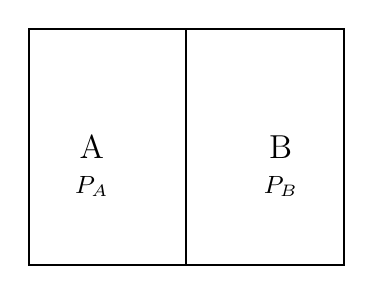
\begin{tikzpicture}[
    chamber/.style={rectangle, draw=black, thick, minimum width=4cm, minimum height=3cm},
    divider/.style={thick},
    label/.style={font=\large},
    pressure/.style={font=\small}
]

% Draw the main chamber
\node[chamber] (chamber) {};

% Draw the vertical divider
\draw[divider] (chamber.center) -- ++(0,1.5cm);
\draw[divider] (chamber.center) -- ++(0,-1.5cm);

% Label chamber sections
\node[label] at ([xshift=-1.2cm] chamber.center) {A};
\node[label] at ([xshift=1.2cm] chamber.center) {B};

% Add partial pressure labels
\node[pressure] at ([xshift=-1.2cm, yshift=-0.5cm] chamber.center) {$P_A$};
\node[pressure] at ([xshift=1.2cm, yshift=-0.5cm] chamber.center) {$P_B$};

\end{tikzpicture}
\end{center}
So, at cont T and const. composition,
\[
d\mu_i = V_i dp
\]
\[
\Delta \mu_i = \mu_i (T, P_i) - \mu_i(T,P) = \int_P^{P_i} V_idp = \int_P^{P_i} \frac{RT}{P} dp = RT \ln{\chi_i}
\]
Basically, any change in the chemical potential means that the only change will occur in the mole fraction and vice-versa.
\[
\mu_i (T,P, \chi_i) = \mu_i(T,P) + RT\ln{\chi_i}
\]
\[
\mu_i = \mu_i^* + RT\ln{\chi_i}
\]
where, $\mu_i^*$ is the reference state, maybe the ideal gas situation. 

\\
This means that suppose we have $P_{i_1} \rightarrow P_{i_2}$, then we have the different refernce state,
\[
\mu_{i_1}  = \mu_{i_2} + RT\ln{\frac{c_{i_2}}{c_{i_1}}}
\]
This is an alternate reference state.
\[
P_i = \frac{n_iRT}{V} = c_iRT
\]
\[
\frac{a_{i_2}}{a_{i_1}} = \frac{\chi_{i_2}}{\chi_{i_1}}
\]
Change in the mixture and not the $G_{mix}$, remember the later is a wrong notation.
So we have ,
\[
\Delta_{mix} G = G_{T,P} +  G_{T,P}^*

\]
\[
= \sum_i n_i\mu_i - \sum_in_i\mu_i^*
\]
\[
= \sum_i n_i(\mu_i^* + RT\ln{\chi_i} - \sum_in_i\mu_i^*
\]
\[
 \Delta_{mix} G = nRT\sum_i \chi_i\ln{\chi_i}
\]
Consider a free adiabetic expansion of ideal gas,,
From $P,V,T \rightarrow P=0, 2V$ this expansion is carried out at const temperature, $dq_{rev} = dw_{rev}$, so we get the entropy change as $nR\ln{2}$

Remember,
\[
\frac{\partial G}{\partial T}|_{P,n} = \Delta_{mix} S
\]
\[
\Delta_{mix} H = \Delta G + T\Delta S = 0
\]
This is an ideal mixture, so there is no enthalpy change in the in the mixing.\\
Find the followings:

\[
\Delta V_{mix} = ?
\]

\[
\Delta A_{mix } = ?
\]
Should there be any change in the entropy of the surrounding? 
\[
\Delta_{mix} S = -nR\sum_i \chi_i\ln{\chi_i}
\]
Since this is a const pressure process, then heat change is the enthalpy change and since enthalpy change is 0, so the process is adiabetic.

Can we look at just the state variables of the process and just conclude if the process be spontaneous?
We just did that!!!\\
\textbf{
Any system that is capable of doing work at const temp and pressure then the spontanaity is for only the non-expansion work.
}\\
\textbf{Question:}
\\
Pure liquid A with vapour pressure $P_A$, assume the vapour to be ideal gas, the $\mu_A = \mu_0 + RT\ln{P_A^*}$, $P_A^*$ is the vapour pressure relative the reference state $P_A^* = \frac{P_A}{P_0}$ , $\mu_A$ chemical potential of the vapour phase. Since the chemical eq. guarantees that the $\mu_A = \mu_{liquid}$ meaning we can use the same ideal gas law can be applied to the liquid, as long as it's in chem eq and the vapour behaves ideally.
\\
Now, if I go from the pure liquid to a mixture of liquid, that might not be solid. I am mixing 2 liquids. I am moving away from the pure state, the eq may not be valid now. 
\[
\mu_{A_{mix}} = \mu_0  + RT\ln{P_{A_{mix}}'}
\]
\[
\mu_{A_{liq}} = \mu_0  + RT\ln{P_{A_{liq}}^*}
\]
mix is the mixture of A and B. 

If we see the change in the chem potential,
\[
\mu_{A_{mix}} - \mu_{A_{pure}} = RT\ln{\frac{P_{A, mix}}{P_{A,pure}}}
\]
\[
P_A' = \frac{P_{A,m}}{P_0}
\]

\[
\frac{P_A'}{P_A^*} = \frac{P_{A,mix}}{P_{A, pure}}
\]

\subsection{Rault's Law}

\begin{center}
    

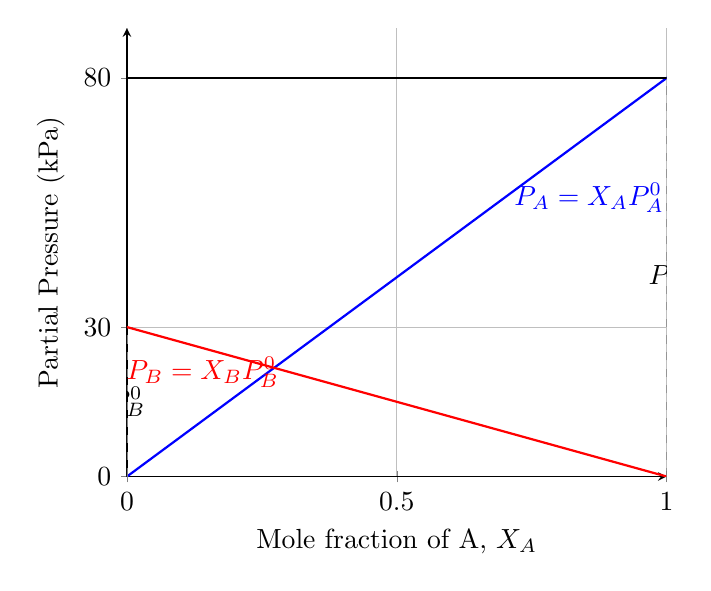
\begin{tikzpicture}
\begin{axis}[
    xlabel={Mole fraction of A, $X_A$},
    ylabel={Partial Pressure (kPa)},
    xmin=0, xmax=1,
    ymin=0, ymax=90,
    xtick={0,0.5,1},
    ytick={0,30,80},
    grid=both,
    axis lines=left,
    smooth]

% Partial pressure curves
\addplot[blue, thick] {80*x}; % P_A = X_A * P_A^0 (P_A^0 = 80 kPa)
\addplot[black, thick] {80};
\addplot[red, thick] {30*(1 - x)}; % P_B = X_B * P_B^0 (P_B^0 = 30 kPa)

% Dashed lines for pure component vapor pressures
\draw[dashed, gray] (axis cs:1,0) -- (axis cs:1,80); % P_A^0
\draw[dashed, gray] (axis cs:0,0) -- (axis cs:0,30); % P_B^0

% Labels for pure component pressures
\node at (axis cs:1,40) {$P_A^0$};
\node at (axis cs:0,15) {$P_B^0$};

% Curve labels
\node[blue, right] at (axis cs:0.7,56) {$P_A = X_A P_A^0$};
\node[red, left] at (axis cs:0.3,21) {$P_B = X_B P_B^0$};

\end{axis}
\end{tikzpicture}
\end{center}
\[
P_{A, mix} = P_{A, pure}\chi_A
\]
\[
\frac{P_A}{P_{A, pure}} = \chi_A
\]


Definition of an Ideal Solution: Such that the chem potential of A summed to the $RT\ln{\chi_A}$

\subsection{Henry's Law}
As $\chi_B \rightarrow0$,

\[
P_B \propto \chi_B
\]

Think of a solution in a closed vessel with components A and B, a monogeneous mix, the rate of evaporation of A will be related to the number of molecules of A or the mole fraction of A  ie. $\chi_A$
\[
\text{Rate of Evaporation} = k\chi_A
\]
\[
\text{Rate of Condensation} = k'P_A
\]
\[
P_A = \frac{k}{k'}\chi_A
\]
Interactions deviate from the ideality, the molecules on the surface are drastically different from the bulk molecules.

So, this law also makes you think about the ideality of the solution.

\begin{enumerate}
    \item The solute is not volatile, meaning you will only see the solvent.
    \item The dissolved solute will not be a part of the solid solvent.
\end{enumerate}



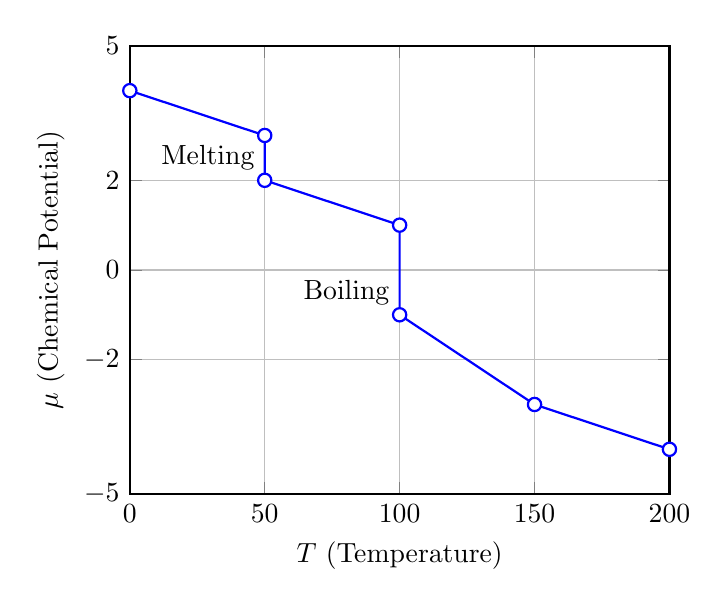
\begin{tikzpicture}
    \begin{axis}[
        xlabel={$T$ (Temperature)},
        ylabel={$\mu$ (Chemical Potential)},
        grid=major,
        thick,
        domain=0:200,
        samples=100,
        ymin=-5, ymax=5,
        xmin=0, xmax=200,
        xtick={0,50,100,150,200},
        ytick={-5,-2,0,2,5},
    ]
    
    % Chemical potential decreasing with steps at phase transitions
    \addplot[
        blue, thick, mark=*, mark options={scale=1.2, fill=white}
    ] coordinates {
        (0,4) (50,3) (50,2) (100,1) (100,-1) (150,-3) (200,-4)
    };
    
    % Labels for melting and boiling points
    \node at (axis cs:50,2.5) [anchor=east] {Melting};
    \node at (axis cs:100,-0.5) [anchor=east] {Boiling};
    
    \end{axis}
\end{tikzpicture}

\textbf{Nature of the graph:} $RT\ln{\chi_A}$ here $\chi_A \leq 1$ meaning the chemical potential of the solvent of the mixture will always be less than the pure solvent.

\[
\text{Change in the Temp for freezing and boiling } \propto \chi
\]

\begin{figure}
    \centering
    \includegraphics[width=0.5\linewidth]{images/chem_pot_collegative.png}
    \caption{Caption}
    \label{fig:enter-label}
\end{figure}

\[
\mu_{A,gas} = \mu_{A, liquid}
\]
\[
\mu_{A,gas}^* = \mu_{A,liquid}^* + RT\ln{\chi_A}
\]

\[
\ln{\chi_A} = \frac{\mu_{A,gas}^* - \mu_{A,liquid}^*}{RT} = \frac{\Delta G_{vap}}{RT}
\]

\[
\frac{d}{dt}(\ln{\chi_A}) = \frac{1}{R} \frac{d}{dt} \frac{\Delta G_{vap}}{T} = - \frac{\Delta H_{vap}}{RT^2}
\]
\[
\int_0^{\ln{\chi_A}} d(\ln{\chi_A}) = - \int_{T^*}^{T} \frac{\Delta H_{vap}}{RT^2} dT
\]
\[
\implies \ln{1-\chi_B} =  -\frac{\Delta H_{vap}}{R}\{\frac{1}{T^*}- \frac{1}{T}\}
\]
\[
\frac{\partial }{\partial T}(\frac{\Delta G}{T})_P = - \frac{\Delta H}{T^2}
\]
\[
\frac{\partial G}{\partial T}_P = \frac{G-H}{T}
\]

\[
\frac{\partial}{\partial T} \frac{\Delta G}{T} = -\frac{G}{T^2} + \frac{G-H}{T^2} = -\frac{\Delta H}{T^2}
\]

\section{AI Trying to Summerize the Notes by Dr. Debanshu Chowdhury:}

\subsection{Introduction to Thermodynamics}

Albert Einstein once said: ``A law is more impressive the greater the simplicity of its premise and wider its range of applicability. Thermodynamics is the only physical theory that within the framework of its applicability will never be overthrown.''

Thermodynamics is a branch of physics that deals with heat, work, and temperature, and their relation to energy, radiation, and physical properties of matter. The behavior of these quantities is governed by the four laws of thermodynamics which define fundamental physical quantities (temperature, energy, and entropy) that characterize thermodynamic systems.

\subsection{System and Surroundings}

A thermodynamic system is defined as a quantity of matter or a region in space chosen for study. Everything external to the system is called the surroundings.

Systems can be classified as:
\begin{itemize}
    \item \textbf{Open system}: Can exchange both energy and matter with surroundings
    \item \textbf{Closed system}: Can exchange energy but not matter with surroundings
    \item \textbf{Isolated system}: Cannot exchange energy or matter with surroundings
\end{itemize}

The boundary separating the system from its surroundings can be:
\begin{itemize}
    \item \textbf{Real}: Physical barrier
    \item \textbf{Imaginary}: Conceptual demarcation
\end{itemize}

\subsection{State Variables and Equilibrium}

\subsubsection{State Variables}
The state of a thermodynamic system is completely specified by a set of quantities called \textbf{state variables} (also known as state functions or state parameters). Common state variables include:

\begin{itemize}
    \item Pressure ($p$)
    \item Temperature ($T$)
    \item Volume ($V$)
    \item Number of moles ($n$)
\end{itemize}

State variables are path-independent, meaning their change depends only on the initial and final states, not on the path taken between them.

\subsubsection{Types of State Variables}
\begin{itemize}
    \item \textbf{Extensive variables}: Scale with the size of the system (e.g., volume, internal energy, entropy)
    \item \textbf{Intensive variables}: Independent of the size of the system (e.g., temperature, pressure, density)
\end{itemize}

For a one-component, single-phase system, the state can be completely defined by only 2 intensive variables. This is a consequence of the Gibbs' Phase Rule:

\[
F = C - P + 2
\]

Where:
\begin{itemize}
    \item $F$ is the number of degrees of freedom
    \item $C$ is the number of components
    \item $P$ is the number of phases
\end{itemize}

\subsubsection{Equation of State}
An \textbf{equation of state} relates different state variables of a system at equilibrium. The most famous example is the ideal gas equation:

\[
pV = nRT
\]

Where:
\begin{itemize}
    \item $p$ is pressure
    \item $V$ is volume
    \item $n$ is number of moles
    \item $R$ is the universal gas constant (8.314 J/mol·K)
    \item $T$ is temperature in Kelvin
\end{itemize}

\subsubsection{Equilibrium}
A system is said to be in \textbf{equilibrium} when its state variables do not change with time. Types of equilibrium include:

\begin{itemize}
    \item \textbf{Mechanical equilibrium}: No unbalanced forces (uniform pressure)
    \item \textbf{Thermal equilibrium}: Uniform temperature throughout the system
    \item \textbf{Chemical equilibrium}: No net chemical reactions occurring
\end{itemize}

\subsection{Exact and Inexact Differentials}

In thermodynamics, it's crucial to distinguish between exact (state variables) and inexact (path variables) differentials:

\begin{itemize}
    \item \textbf{Exact differentials} (denoted by $d$): Represent changes in state functions. The integral of an exact differential depends only on the initial and final states, not on the path.
    \item \textbf{Inexact differentials} (denoted by $\delta$): Represent path-dependent quantities like heat and work. The integral of an inexact differential depends on the specific path taken.
\end{itemize}

For a function $f(x,y)$, its differential $df$ is exact if:

\[
\frac{\partial}{\partial y}\left(\frac{\partial f}{\partial x}\right) = \frac{\partial}{\partial x}\left(\frac{\partial f}{\partial y}\right)
\]

\subsection{The Laws of Thermodynamics}

There are four fundamental laws of thermodynamics, which cannot be proven but are taken to be inviolable based on empirical evidence:

\subsubsection{Zeroth Law of Thermodynamics}

If two systems are each in thermal equilibrium with a third system, then they are in thermal equilibrium with each other.

Mathematically: If $T_A = T_B$ and $T_B = T_C$, then $T_A = T_C$

This law establishes temperature as a fundamental property and allows for the construction of thermometers. Temperature is a measure of the average kinetic energy of molecular motion in a substance.

\subsubsection{First Law of Thermodynamics}

Energy can neither be created nor destroyed; it can only be converted from one form to another.

For a closed system:
\[
dU = \delta q + \delta w
\]

Where:
\begin{itemize}
    \item $dU$ is the change in internal energy of the system
    \item $\delta q$ is the heat added to the system
    \item $\delta w$ is the work done on the system
\end{itemize}

The total energy of a system is:
\[
E = K + V + U
\]

Where:
\begin{itemize}
    \item $K$ is the macroscopic kinetic energy
    \item $V$ is the macroscopic potential energy
    \item $U$ is the internal energy
\end{itemize}

For a system at rest under no external potential, $E = U$.

It's important to note that while heat and work are path variables, their sum (the change in internal energy) is a state variable.

\subsubsection{Second Law of Thermodynamics}

The entropy of an isolated system never decreases; it either increases or remains constant.

\[
\Delta S \geq 0 \quad \text{(for an isolated system)}
\]

The second law introduces the concept of entropy and defines the direction of thermodynamic processes, establishing the arrow of time.

\subsubsection{Third Law of Thermodynamics}

As the temperature of a system approaches absolute zero, the entropy of the system approaches a minimum value.

\[
\lim_{T \to 0} S = S_0
\]

This law allows us to assign a numerical value to entropy.

\subsection{Work, Energy, and Heat}

\subsubsection{Work}
Work in thermodynamics is defined similarly to classical mechanics:
\[
\delta w = F \cdot dx
\]

For volume change work (expansion/compression):
\[
\delta w = -p \cdot dV
\]

The negative sign indicates that when a system expands ($dV > 0$), it does work on the surroundings ($\delta w < 0$).

\subsubsection{Energy}
Energy is the capacity of a system to do work. Examples include:
\begin{itemize}
    \item Compressed gas
    \item Wound spring
    \item Elevated weight
    \item Hot water
\end{itemize}

\subsubsection{Heat}
Heat is energy transferred due to temperature differences. While work and heat are both forms of energy transfer, they differ fundamentally:
\begin{itemize}
    \item \textbf{Work}: Organized, directional transfer of energy
    \item \textbf{Heat}: Disorganized, random transfer of energy
\end{itemize}

\subsection{Reversible and Irreversible Processes}

\subsection{Reversible Process}
A process that can be reversed by an infinitesimal change in a variable, returning both the system and the surroundings to their initial states.

For a reversible isothermal expansion of an ideal gas:
\[
w_{rev} = -nRT\ln\frac{V_f}{V_i}
\]

\subsubsection{Irreversible Process}
Any process that is not reversible. All real processes are irreversible.

For an irreversible isothermal expansion of an ideal gas:
\[
w_{irr} = -p_{ext}(V_f - V_i)
\]

It can be shown that:
\[
|w_{rev}| \geq |w_{irr}|
\]

This means a reversible process extracts the maximum possible work from a system.

\subsection{Joule Expansion}

Joule (free) expansion is an irreversible process in which a gas expands into a vacuum. During this process:
\begin{itemize}
    \item No work is done: $\delta w = 0$ (expansion against zero pressure)
    \item No heat is transferred: $\delta q = 0$ (adiabatic process)
\end{itemize}

Therefore, from the first law:
\[
dU = \delta q + \delta w = 0
\]

For an ideal gas, the internal energy depends only on temperature, so $\Delta T = 0$ during Joule expansion. 

For a real gas, however, the temperature may change due to intermolecular forces.

\subsection{Heat Capacity}

Heat capacity is the amount of heat required to raise the temperature of a substance by one unit.

\subsubsection{Heat Capacity at Constant Volume}

\[
C_V = \left(\frac{\partial U}{\partial T}\right)_V = \left(\frac{\delta q}{\delta T}\right)_V
\]

For an ideal gas:
\[
C_V = \frac{f}{2}nR
\]

Where $f$ is the number of degrees of freedom.

\subsubsection{Heat Capacity at Constant Pressure}

\[
C_p = \left(\frac{\partial H}{\partial T}\right)_p = \left(\frac{\delta q}{\delta T}\right)_p
\]

For an ideal gas:
\[
C_p = C_V + nR
\]

This shows that $C_p > C_V$ for any substance, as some additional energy is needed at constant pressure to perform expansion work.

\subsection{Enthalpy}

Enthalpy ($H$) is a thermodynamic property defined as:
\[
H = U + pV
\]

The differential form is:
\[
dH = dU + pdV + Vdp
\]

At constant pressure:
\[
dH = dU + pdV = \delta q_p
\]

This makes enthalpy particularly useful for analyzing processes that occur at constant pressure, such as most chemical reactions.

For a reaction involving gases:
\[
\Delta H = \Delta U + \Delta n_g RT
\]

Where $\Delta n_g$ is the change in the number of moles of gas.

\subsection{Adiabatic Processes}

An adiabatic process is one in which no heat is exchanged with the surroundings ($\delta q = 0$).

For an adiabatic process:
\[
dU = \delta w = -pdV
\]

For an ideal gas undergoing a reversible adiabatic process:
\[
pV^\gamma = \text{constant}
\]

Where $\gamma = C_p/C_V$ is the heat capacity ratio.

Temperature and volume are related by:
\[
TV^{\gamma-1} = \text{constant}
\]

Temperature and pressure are related by:
\[
T p^{(1-\gamma)/\gamma} = \text{constant}
\]

\subsection{Joule-Thomson Effect}

The Joule-Thomson effect describes the temperature change of a gas when it is allowed to expand through a porous plug or valve while being thermally insulated so that no heat is exchanged with the environment.

\subsubsection{Joule-Thomson Coefficient}

The Joule-Thomson coefficient is defined as:
\[
\mu_{JT} = \left(\frac{\partial T}{\partial p}\right)_H
\]

It measures the temperature change per unit pressure drop at constant enthalpy.

For an ideal gas: $\mu_{JT} = 0$ (no temperature change)

For a real gas:
\begin{itemize}
    \item $\mu_{JT} > 0$: Gas cools during expansion (intermolecular attraction dominates)
    \item $\mu_{JT} < 0$: Gas warms during expansion (intermolecular repulsion dominates)
\end{itemize}

The Joule-Thomson experiment is an isenthalpic process:
\[
H_2 = H_1
\]
\[
U_2 + p_2V_2 = U_1 + p_1V_1
\]

\subsubsection{Inversion Temperature}

The temperature at which $\mu_{JT} = 0$ is called the inversion temperature. Above the inversion temperature, a gas warms upon expansion; below it, the gas cools.

\subsection{Thermochemistry}

Thermochemistry deals with the heat changes accompanying chemical reactions.

\subsubsection{Standard Enthalpy of Formation}

The standard enthalpy of formation ($\Delta H_f^°$) is the enthalpy change when one mole of a compound is formed from its elements in their standard states at 298.15 K and 1 bar pressure.

By convention:
\[
\Delta H_f^°(\text{element in its standard state}) = 0
\]

\subsubsection{Enthalpy of Reaction}

The enthalpy change for a reaction can be calculated using Hess's Law:
\[
\Delta H_{rxn} = \sum \Delta H_f^°(\text{products}) - \sum \Delta H_f^°(\text{reactants})
\]

This reinforces the state function property of enthalpy, as the overall enthalpy change depends only on the initial and final states, not on the pathway.



\end{document}
